
\chapter{Código Network Evaluation}\label{chap:CNeval}{

Until this point the report motivated and descrobed the design of Código network, and evaluated the performance of the developed smart-contracts. As with any other distributed system, it is critical to measure Código network performance and evaluate how it stands against other competing technologies. Therefore, in this section the attention is shifted towards evaluating the efficiency of the developed framework in distributing a file from the developer to the rest of the users. The performance of the system is evaluated experimentally and is compared against the Client-Server model and the BitTorrent protocol. The comparison is based on the concept of average delay. Average delay is a measure that expresses the average time required for $k$ users to simultaneously download the same firmware. Additionally we explore the issue of redundancy and overheads in firmware distribution.

\section{Performance Experiments}{
\subsection{Experiment Setting}{

To evaluate the performance of the network we consider the following experiment setting. A single user creates a new firmware and $k$ users simultaneously download it. The firmware size is 10MB.  For this set of experiments all nodes are in the same Local Area Network and have 0\% packet loss and minimal latency. In particular, since all the communications are within the localhost, we have only the latency associated with the system processing the request. All the experiments are executed in the Google Cloud Compute engine using a virtual machine with 64 CPUs and 240 GB memory, and Ubuntu 16.04 LTS as the operating system.

Our generic simulation algorithm is shown in Algorithm \ref{alg:simulation}. There the functions $upload\_file()$ and $download\_file()$  depend on the framework. For example, for the Client-Server model, the $upload\_file()$ would be starting the file distribution server and $download\_file()$ would be making an HTTP request to that server. Furthermore, the $download()$ function in the simulation is used in asynchronous manner to capture the idea of multiple nodes downloading the same file at the same time. In the $download()$ function we additionally may use mutexes to avoid data racing condition, if the append function is not thread safe in the language used to implement the logic of the simulation. For example in Python (used for Client-Server simulation) append is thread safe whereas in Golang (used for IPFS simulation) we use the Golang channels. Algorithm \ref{alg:simulation} is used by Algorithm \ref{alg:simulationFull} to execute the simulation for $k$ users where $k \in [1,120]$ 

\begin{algorithm}
\caption{Core Simulation}\label{alg:simulation}
\begin{algorithmic}[1]

\Function{Simulation\_Core}{users}
    \State {$upload\_file()$}
    \State $delay[]$
    \Function{download}{}
        \State {$start$ $\gets$ {$now$}}
        \State {$download\_file()$}
        \State {$end$ $\gets$ {$now$}}
        \State {$delay[]$ $\gets$ $delay[]$ + {$(end - start)$}}
    \EndFunction
    
    \For{$user \gets 1$ to $users$}                    
        \State \text{async} $DOWNLOAD()$
    \EndFor
    \State \text{Wait for all calls to finish}
    \State {$calculate\_statistics(delay)$}
    \EndFunction
    \end{algorithmic}
\end{algorithm}

\begin{algorithm}
\caption{Simulation Procedure}\label{alg:simulationFull}
\begin{algorithmic}[1]

    \For{$k \gets 1$ to $max\_users$}                    
        \State $Simulation\_Core(k)$
    \EndFor
\end{algorithmic}
\end{algorithm}

In the $calculate\_statistics(delay)$, we calculate the \textit{average delay} ($\bar{d}$) in retrieving the file as follows:

\begin{align*}
\bar{d} = \frac{\sum_{i=1}^{k}{t_i}}{k}
\end{align*}

where 

\begin{itemize}
\item $t_i$ is the time that it took user $i$ to download the file.
\item $k$ is the number of users that simultaneously retrieve the file.
\end{itemize}

Similarly, we calculate and use other useful metrics such as the standard deviation of the delay, the minimum and the maximum. 

To implement the simulations the following tools were utilized:
\begin{enumerate}
\item \textbf{The IPTB framework} \footnote{Forked IPTB: \url{https://github.com/davinci26/iptb}}: The official IPTB framework was forked and expanded to meet our simulation requirements. The simulation flow and the calculations above were implemented in IPTB. The IPTB framework spawns multiple IPFS nodes in a single machine and each node is unaware of the existence of the rest of the local nodes. When the simulation starts, nodes asynchronously start downloading the file. The results are combined together when all nodes download the file. Our simulation framework is currently under code review and will be integrated in the official IPTB framework to measure the performance of IPFS \footnote{Pull request: \url{https://github.com/ipfs/iptb/pull/65}}.
\item \textbf{BitTorrent simulation tool \footnote{BitTorrent Simulator: \url{https://github.com/thejosh223/cs198mojo/tree/master/PeerSimCode/Peersim-BitTorrent}}}: This tool utilizes the P2P simulation library \cite{p2p09-peersim}. The simulation tool is a lightweight implementation of the BitTorrent protocol that does not actually transfer the file but simulates the transfer as a set of messages. Note that the BitTorrent simulation is based on fixed time intervals set to 1 second, as a result all the results produced by the simulation have an error margin of $\pm$ 0.49 seconds
\item \textbf{Client-Server Simulator}: This consists of a pair of Python programs responsible for implementing a Server and a set of $k$ clients. The tailor made Python flask server \cite{flask} responds to HTTP requests with a 10MB file. The set of $k$ clients  are implemented as different threads. The client program spawns $k$ threads that request the file simultaneously from the server.
\end{enumerate}
}
An important detail for the P2P systems, namely IPFS and BitTorrent, is that users close their IPFS and BitTorrent clients when all the other users in the system have finished downloading the firmware. This is a strong assumption that works in favor of performance for the decentralized systems, as the users who download the file early do not abort the protocol but remain as file seeders. 

\subsection{Results}{

In terms of performance the client-server is able to outperform both decentralized systems in file distribution. This is illustrated in Figure \ref{fig:CSPerf} that shows that distributing a single file to 100 users takes ~2.491 seconds. The main issue with this approach is that by definition the cloud server is single point of failure in the system. As a result, the distribution of the firmware is limited to the ability of the manufacturer to afford Cloud computing resources. To put things into perspective the cost of the instance used to perform the simulations is \$ 20,717.04 per year according to the Google Cloud Billing plan. Additionally, as the cost of vertical scaling in web applications increases exponentially, sustaining even higher number of users would result in exponentially higher costs.

\begin{figure}[!htb]
\centering
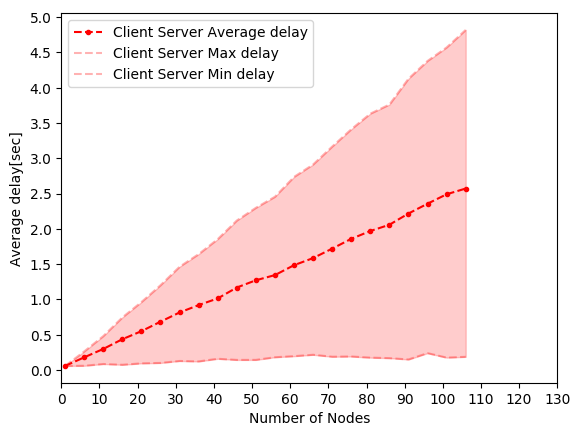
\includegraphics[width=\textwidth]{./results/client-server.png}
\caption{Average delay in downloading a single 10MByte file from a Python Flask server, as a function of the number of users, that want to download the file. Each data point refers to a single execution of Algorithm \ref{alg:simulation}.}
\label{fig:CSPerf}
\end{figure}

IPFS network which constitutes the framework that Código network uses to distribute firmware to the users has a solid performance that deteriorates as the numbers of users increases. The first observation that should be made is that the average time required to download the same file, when 100 nodes want the file, using IPFS is 22.9 times slower than the client-server model. The more worrying part is not that IPFS is orders of magnitude slower than client-server, but that the average delay is increasing almost linearly as the number of nodes increases. Intuitively we expect that, in a P2P system as the number of nodes increase, both the number of seeders and the number of leechers increase and the load is balanced among the users. This should guarantee a better performance at scale. Figure \ref{fig:IPFSPerf} illustrates the performance of IPFS network as the number of users requesting the file increases.

\begin{figure}[!htb]
\centering
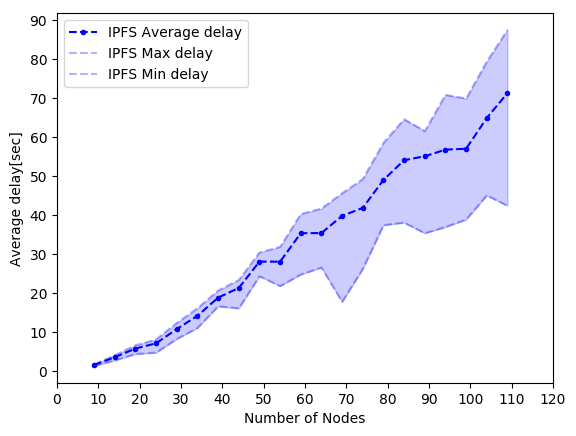
\includegraphics[width=\textwidth]{./results/ipfs-perf.png}
\caption{Average delay in downloading a single 10MByte file using the IPFS network. Even though it is a P2P network it seems that the average time required to download the file increases as the number of users increases. Each data point refers to a single execution of Algorithm \ref{alg:simulation}}
\label{fig:IPFSPerf}
\end{figure}

To understand why our intuition was incorrect, we decided to delve deeper into the implementation of the IPFS Bitswap protocol that is responsible for the file distribution. We discovered that the current design of block swapping has a flaw that causes the performance deterioration. In particular what is happening now is that nodes that want to download a file share to the network a \textit{wantlist} of the blocks they need. Remember, each file in IPFS is split in a set of blocks. Then other seeders, see the \textit{wantlist} of other users and send them the block. For example, if Alice wants to download a file that consists of four blocks (b1,b2,b3,b4) she will publish a wantlist that consists of $[b1,b2,b3,b4]$. Then users Bob and Charlie who already have the blocks and want to participate in the exchange will start sending Alice raw data.

At the time of receiving data from Bob and Charlie, Alice does not know which block she receives. As a result, she will wait until the transmission is over and then calculate the hash of the received bytes. If the hash matches one of the blocks in the wantlist she removes it from her wantlist. The problem is that Alice does not know which block she receives before the transmission is over. Additionally, Bob does not know that Charlie is also sending a block to Alice and vice versa. As a result as the number of users increase, Alice would spend her bandwith in publishing her wantlist to multiple nodes and receiving duplicate blocks from other nodes. This result is shown in Figure \ref{fig:IPFSDups} which illustrates the total number of duplicate blocks transmitted in the network in terms of the nodes participating in the exchange of a single file. It can be observed that there is a linear increase in the number of duplicate blocks as the number of users in the swarm increase. This lack of coordination between block senders and receivers is the reason behind the performance deterioration of IPFS as the number of users interested in a single file increase.

\begin{figure}[!htb]
\centering
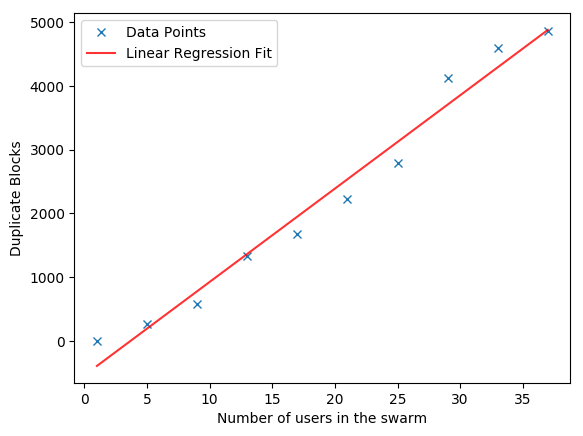
\includegraphics[width=\textwidth]{./results/ipfs_duplicates.png}
\caption{Number of duplicate blocks exchanged in the IPFS newtwork as a function of number of users in the swarm. It can observed that as the number of nodes interested in a single file increases then more duplicate blocks are transmitted. Due to the lack of communication between network users, nodes end up wasting resources to exchange duplicate blocks.}
\label{fig:IPFSDups}
\end{figure}

The content distribution is a crucial component of Código network. The fact that IPFS performance is way worse than the Client-Server model is not a major concern for Código network. One of the motivations for designing a decentralized firmware distribution network was to enable a robust model for open-source development of firmware. This is not possible under the Client-Server model, as the operator of the server is an implicit trusted party and a single point of failure. Additionally, another advantage of IPFS against Client-Server model is that it does not require an Internet connection to work. In a network of multiple IoT devices connected via WLAN, if one of the devices has the file then it can distribute it via WLAN to the rest. Furthermore, we simulated a situation where all devices are in the WLAN and share the firmware. However, consider the case in which the distribution server is the US and the nodes requesting the file are in Europe. IPFS would prioritize devices with better connection and thus have a better performance under those conditions. This comes from the fact that IPFS uses the "tit-for-tat" mechanism. For example, let Alice be in the EU, Bob in the USA and Charlie also in EU. Then Alice would have better connection speed with Charlie (EU) compared to Bob (USA). As a result, due to the incentives of the protocol, Alice would engage in more block transactions with Charlie because he is uploading more data at a fixed time interval.

The last question that we chose to address in this project is how IPFS compares against BitTorrent in terms of performance. As both systems are decentralized this comparison will be more meaningful. It can be observed that BitTorrent is on average slower than IPFS and by a big margin. Additionally, the BitTorrent protocol (different BitTorrent clients can optimize around this problem) is not fair towards the users, as the difference between the minimum and the maximum download time could be different by orders of magnitutde. Figure \ref{fig:BitTorrentPerf} demonstrates the performance of BitTorrent protocol in distributing a single file to multiple nodes as the numbers of nodes increases. However, as the number of nodes increases, give the performance of IPFS we assume that there exists a sufficiently large number of nodes for with BitTorrent will outperform IPFS.

\begin{figure}[!htb]
\centering
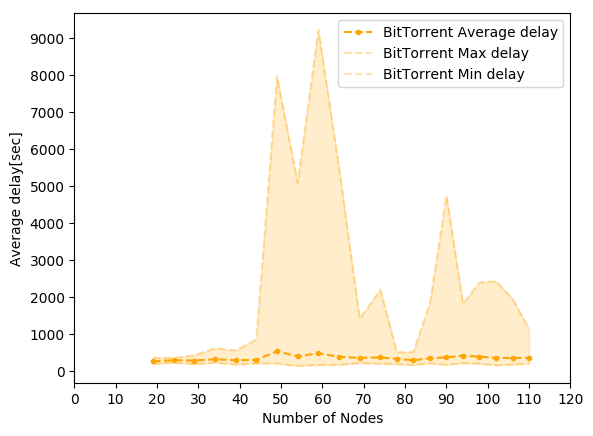
\includegraphics[width=\textwidth]{./results/BitTorrent.png}
\caption{Average delay in downloading a single 10MByte file using the BitTorrent network. The BitTorrent protocol seems not to be affected on average by the number of users in the swarm.}
\label{fig:BitTorrentPerf}
\end{figure}

The aforementioned comparison between content distribution frameworks is summarized in Table \ref{tab:all_comp} in which the average, std, median, min, max delay are presented for100 users trying to simultaneously download a single 10 MByte file.

\begin {table}[htb!]
\caption {Comparison between Client-Server model, BitTorrent and IPFS in the distribution of a single file to 100 users} \label{tab:all_comp} 
\begin{center}
 \begin{tabular}{|c| c|c |c | c| c |}
 \hline
  & \multicolumn{5}{|c|}{Delay[sec]} \\
 \hline
 Model & Average& Std & Median & Min & Max \\ [0.5ex] 
 \hline
  Client-Server & 2.491 & 1.259 & 2.549 & 0.176 & 4.571 \\
  \hline
  BitTorrent & 331.489 & 82.552 & 330.0 $\pm$ 0.49 & 180.0 $\pm$ 0.49 & 590.0 $\pm$ 0.49 \\
  \hline
  IPFS & 57.053 & 5.958 & 57.938 & 38.910 & 69.931 \\
  \hline
\end{tabular}
\end{center}
\end {table}

}
}
}